\chapter{Measuring the Gravitational Constant}

%TODO Changes:
% - don't have them build the balance.
% - have better way of taking video of moving laser, transferring to computer. Consider having computers with webcams.

Gravity is the least understood of the fundamental forces, and it is the one that is most easily noticed by humans. Part of the reason for this second part is that gravity is weak enough that we can easily push and move against it (for example, walking or launching a rocket). Compared with the electromagnetic bonds that are holding molecules together or the nuclear forces that hold atomic nuclei, gravity is extremely weak.

If it is universal, though, we should be able to measure the gravitational attraction between any two massive objects, if we are very careful and have sensitive equipment. In this lab, we will measure the gravitational force between lead spheres and use that to find the Newtonian constant of gravitation, $G$, which is a measure of how strong, in general, the force of gravity is.

\section{Learning goals}

\begin{itemize}
	\item Follow the procedure of an important physical measurement.
	
	\item Identify sources of statistical and systematic error.
	
	\item Demonstrate an ability to make careful measurements.
\end{itemize}

\textbf{Rubrics rows to be assessed:} D4, D8, F1, F2, G1, G2, G4.

\section{Scientific Background}

In 1798, Henry Cavendish completed his measurements of ``the density of Earth'' using a
simple yet extremely sensitive apparatus: a torsion balance. He placed a small lead sphere
of mass $m = 0.73\:$kg at each end of a wooden rod, which was suspended horizontally.
Two large lead spheres, each of mass $M = 159\:$kg, were fixed in place, at a distance $R =
23\:$cm from each of the smaller spheres. When the torsion balance was released and
allowed to move freely, the lead spheres would be attracted by the gravitational force according to Newton's law of universal gravitation,
\begin{equation}\label{cav:eq:newtons-grav}
 F = G \frac{M m}{R^2} \,.
\end{equation}
To protect the balance from air currents and temperature changes, Cavendish placed it in
a closed room (Fig.~\ref{cav:fig:original-setup}), appropriately equipped for remote operation and reading of the
torsion angle.

\begin{figure}
	\centering
	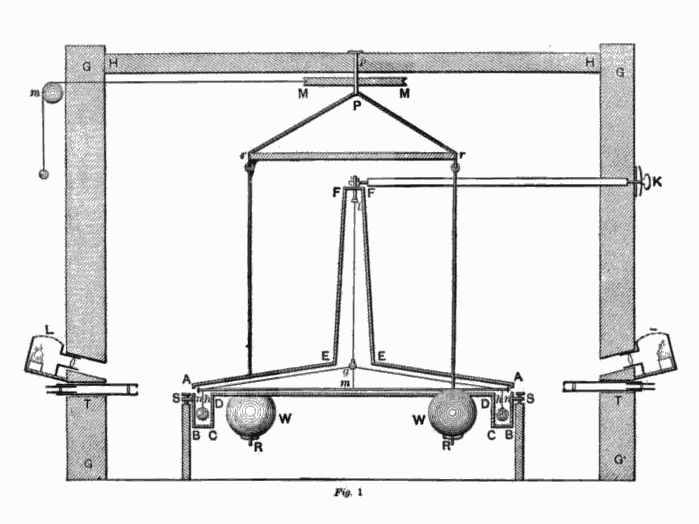
\includegraphics[width=\textwidth]{cavendish/Cavendish_Experiment}
	\caption{Henry Cavendish's sketch of his experimental setup.}\label{cav:fig:original-setup}
\end{figure}

While Cavendish's main objective was the measurement of the density of Earth, in fact
he had performed a measurement of the Gravitational constant $G$ to a remarkable
accuracy ($\approx 1\%$).

High precision torsion balances are still used nowadays to test fundamental principles of
general relativity (the equivalence of the inertial and gravitational mass) and possible
deviations of the Newton’s law of gravitation. In this lab, you will measure the
Gravitational constant with a modern version of the Cavendish torsion balance.

\section{Apparatus and Theory}\label{cav:sec:apparatus}

The setup and measurement of the Gravitational constant is conceptually straightforward (Fig.~\ref{cav:fig:setup-booms}). A boom
with two small, identical lead spheres (labeled `A' in the figure) of mass $m$ is suspended by a thin tungsten
wire. Since the masses are identical, the system is in equilibrium under the Earth
gravitational field. At a certain moment, two large lead spheres (B) of mass $M$ are placed
close to the A spheres.

\begin{figure}
	\centering
	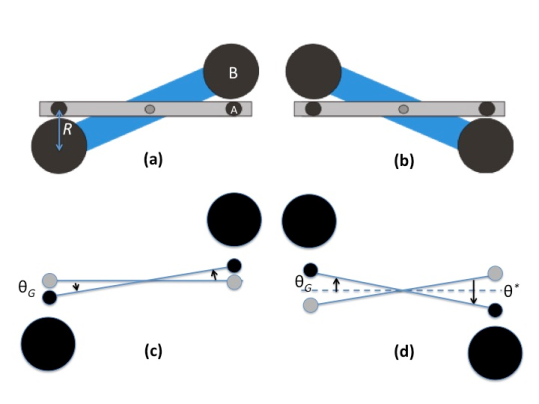
\includegraphics[width=0.7\textwidth]{cavendish/tel-rp2111-booms}
	\caption{A torsion balance. In (a) and (b), top view of the Cavendish balance with two
		symmetric configurations of the lead spheres. In (c) and (d), the corresponding
		equilibrium positions and rotation angles.}\label{cav:fig:setup-booms}
\end{figure}

The gravitational force between spheres A and B is given by Eq.~\ref{cav:eq:newtons-grav}. This force induces a torque $\tau_G$ on the boom which starts to rotate. From the laws of
physics, the torque is given by
\begin{equation}
 \tau_G = 2 F_G d \,
\end{equation}
where $d$ is the distance to the center of A from the center of the boom (the factor 2 comes
from the fact that there are two B spheres each exerting a force $F_G$). The suspending
wire, which is fixed at its top end, is twisted by the rotation of the boom (Fig.~\ref{cav:fig:torsion}), and
``tries'' to recover its initial position by a counter-torque $\tau_w$. For a small rotation angle $\theta$,
$\tau_w$ is proportional to $\theta$,
\begin{equation}
 \tau_w = k \theta\,,
\end{equation}
where the torsion constant $k$ depends on the wire's material and dimensions.

\begin{figure}
	\centering
	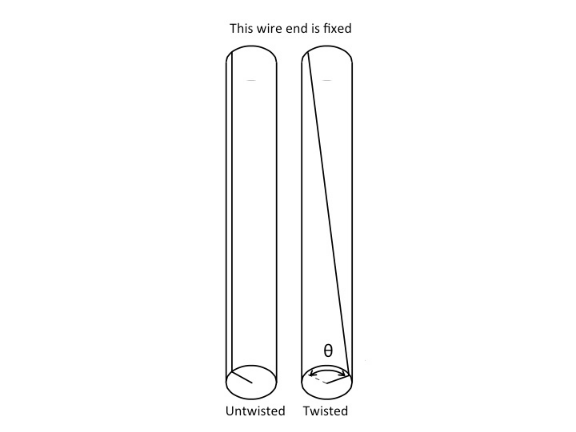
\includegraphics[width=0.8\textwidth]{cavendish/torsion-balance}
	\caption{Twisted wire of a torsion balance.}\label{cav:fig:torsion}
\end{figure}

A new equilibrium position is achieved when the boom has rotated by an angle $\theta_G$ (Fig.~\ref{cav:fig:setup-booms}(c)) such that the two torques equilibrate themselves, so
\begin{equation}\label{cav:eq:equal-taus}
\tau_G = \tau_w \,.
\end{equation}
From Eqs.~(\ref{cav:eq:newtons-grav}--\ref{cav:eq:equal-taus}), the gravitational constant is obtained:
\begin{equation}\label{cav:eq:final-g}
G = \frac{k \theta_G R^2}{2 M m d}\,.
\end{equation}

The symmetry of the torsion balance can be exploited to perform a more precise
measurement of rotation angle $\theta_G$ (which is very small). After the boom has reached the
equilibrium in the Fig.~\ref{cav:fig:setup-booms}(c) configuration, the B spheres are placed in the symmetric position of Fig.~\ref{cav:fig:setup-booms}(b), which results in a new equilibrium position as in Fig.~\ref{cav:fig:setup-booms}(d).
Thanks to the symmetry of the apparatus, the rotation angle $\theta_\textrm{rotation}$ between the two
configurations is simply twice the angle $\theta_G$. With the Cavendish balance described in
Section~\ref{cav:sec:measurement}, you will measure $\theta_\textrm{rotation}$ and then use the following equation to find $\theta_G$:
\begin{equation}\label{cav:eq:theta-g}
 \theta_G = \theta_\textrm{rotation} / 2 \,.
\end{equation}

When performing the experiment, you will notice that the torsion balance undergoes
harmonic oscillations around its equilibrium position. The dampening of the oscillations
(that is, the decrease of their amplitude with time) is due primarily to air dragging against
the boom. The period $T$ of the oscillations depends on the torsion constant $k$ according to
\begin{equation}\label{cav:eq:k}
 k = 2 m d^2 \left( \frac{2 \pi}{T} \right)^2 \,.
\end{equation}
Note that the quantity $2 m d^2$ is the \textit{moment of inertia} of the A spheres.

\section{Procedure: Measurement of $\bm{G}$ with the Cavendish Balance}\label{cav:sec:measurement}

You will perform a measurement of the Gravitational constant using data taken with a
computerized Cavendish balance (Fig.~\ref{cav:fig:comp-setup}). The apparatus is placed on a wooden box filled
with sand which helps in dampening vibrations (of the building, when you walk close to
the apparatus, etc.). The rotation angle is measured by a ``differential capacitive sensor''
which provides a more stable and convenient way of recording when compared to other
methods (e.g. using a laser). The apparatus is extremely sensitive and requires several
hours of preparation. For this reason, it is not possible to set it up and take good data
during a standard two-hour lab session. Thus, you will find the apparatus ready for the
measurements, which will be performed by the TA by moving the B spheres in the two
configurations of Fig.~\ref{cav:fig:setup-booms}. You will notice that after the TA has moved the spheres, the
boom will start to oscillate and it will take about one hour for the oscillations to dampen
around a new equilibrium position. The TA will then provide you with the data after the
session. Sometimes the data collected during your session will not be of good enough
quality for the measurement (this is indeed a very difficult experiment and we are trying
to do it while you walk around the room causing vibrations), and in such case you will
be provided a set of data from another session. An example of data is given in Fig.~\ref{cav:fig:data}
(your data will be significantly noisier).

\begin{figure}
	\centering
	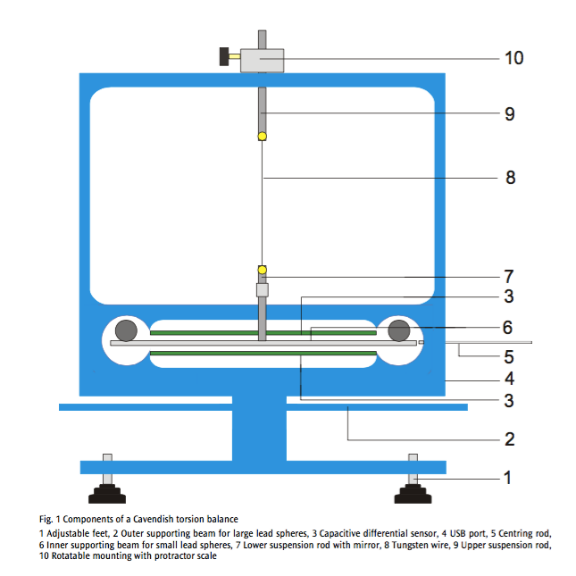
\includegraphics[width=\textwidth]{cavendish/tel-rp2111-setup}
	\caption{The computerized Cavendish balance.}\label{cav:fig:comp-setup}
\end{figure}

\begin{figure}
	\centering
	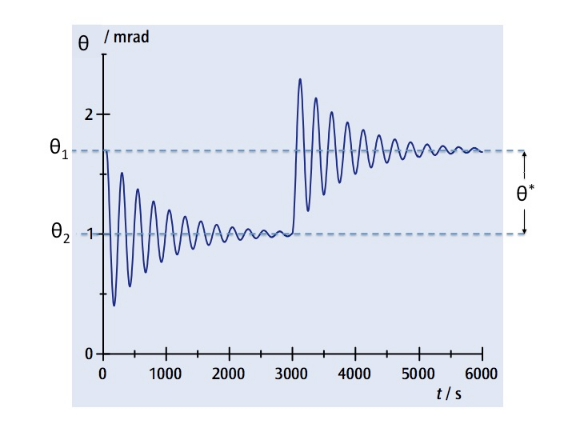
\includegraphics[width=0.8\textwidth]{cavendish/tel-rp2111-example-data}
	\caption{Example of data from the Cavendish balance.}\label{cav:fig:data}
\end{figure}

By analyzing the data, you can determine the Gravitational constant with the following
procedure:
\begin{enumerate}
	\item Measure the period $T$ of oscillation (e.g. by measuring the time between two
	consecutive maxima of the damping oscillations), and determine $k$ using Eq.~(\ref{cav:eq:k}). For a more
	accurate measurement of $T$, measure the time corresponding to several
	oscillations and divide it by the number of oscillations. Use Fig.~\ref{cav:fig:geo} for the values
	of the masses and the geometrical parameters.
	
	\item Measure the rotation angles $\theta_1$ and $\theta_2$ corresponding to the equilibrium positions
	of the first and second oscillation, respectively (see Fig.~\ref{cav:fig:data}). Try various ways to measure the rotation angles (e.g. fitting by eye an horizontal line; sum the
	maxima and minima of consecutive oscillations). You can then calculate
	\begin{equation}
	\theta_\textrm{rotation} = \abs{\theta_1 - \theta_2}
	\end{equation}
	and use Eq.~(\ref{cav:eq:theta-g}) to derive $\theta_G$.
	
	\item Determine the gravitational constant G using Eq.~(\ref{cav:eq:final-g}) and compare your result with its nominal value.
	
	\item Note that the mathematical procedure given here makes some assumptions about what is important to include. Discuss with your group to identify those assumptions and report these in your report.
\end{enumerate}

\begin{figure}
	\centering
	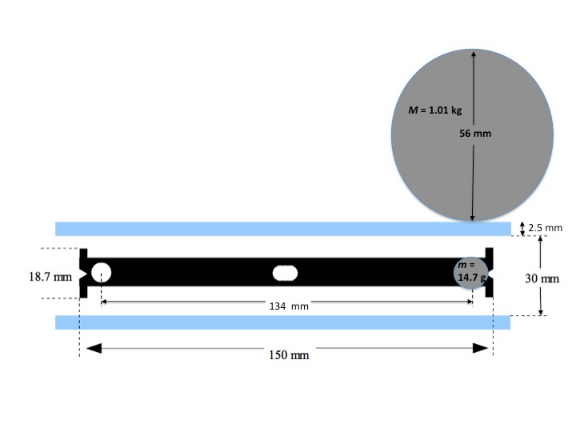
\includegraphics[width=\textwidth]{cavendish/tel-rp2111-geometry}
	\caption{Geometry of the Cavendish balance and lead spheres masses.}\label{cav:fig:geo}
\end{figure}

\section{Procedure: Build the Cavendish Balance}

While the computerized Cavendish balance is acquiring data, you will build and calibrate
a similar apparatus. This part of the lab will give you a deeper understanding of the
Cavendish balance, and a hands-on experience on the extreme sensitivity of the
apparatus. A description of the PASCO balance and instructions are given in the manual in Appendix~\ref{cha:pasco-cavendish}.
Read pages 1--3 of the manual and familiarize yourself with the different components of
the balance.

\begin{enumerate}
	\item First, mount the thin tungsten wire which will be used to suspend the
	pendulum bob. The mounting mechanism is shown in Figs.~\ref{cav:fig:pasco-block}--\ref{cav:fig:pasco-assembly}. A good eye,
	cooperation within you group, and patience is required for this step; be careful in
	handling the wire since it can break (and probably will until you get enough
	practice).
	
	\item To install the wire, screw the small aluminum block onto the tab as in Fig.~\ref{cav:fig:pasco-block} (you
	need to assemble two of these pieces).
	
	\item Mount one of them on the brass rod (torsion wire head) as in Fig.~\ref{cav:fig:pasco-assembly}.
	
	\item Cut $\approx 50\:$cm of wire from the spool; be careful in keeping the wire straight
	avoiding kinks.
	
	\item Take one end of the wire, slide it between the aluminum block and the plate
	(slightly loosen the screw to let the wire in) and make a loop around the screw;
	tighten the screw while keeping the wire (and the aluminum block) straight.
	
	\item Take the other end of the wire and do the same with the other mounting piece; the
	length of the wire between the two mounting screws must be $37.5\:$cm (Fig.~\ref{cav:fig:pasco-assembly}).
	
	\item Thread the wire through the shaft of the Cavendish apparatus (you may need the
	help of a thin screwdriver to slide the mounting piece in).
	
	\item Using the zero adjust knob (see PASCO manual), align the bottom tab with the
	face of the pendulum bob.
	
	\item Tighten the screw on the top of the balance to secure the torsion wire head.
	
	\item Attach the bottom tab to the pendulum bob using the Philips screw.

\end{enumerate}

\begin{figure}
	\centering
	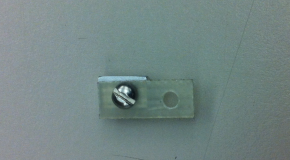
\includegraphics[width=0.5\textwidth]{cavendish/pasco-block}%
	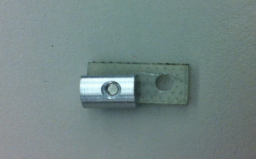
\includegraphics[width=0.45\textwidth]{cavendish/pasco-tab}
	\caption{Wire mounting pieces, aluminum block and tab.}\label{cav:fig:pasco-block}
\end{figure}

\begin{figure}
	\centering
	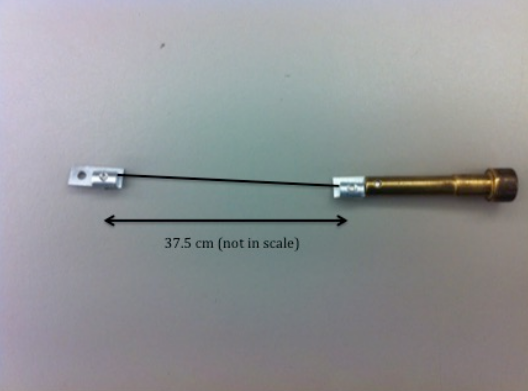
\includegraphics[width=0.7\textwidth]{cavendish/pasco-assembly}
	\caption{Assembly of torsion wire.}\label{cav:fig:pasco-assembly}
\end{figure}

Also, check the Section ``Maintenance'' of the PASCO manual which provides a
description of a similar procedure using a torsion ribbon.

Once you have successfully completed this step, you can proceed to leveling the
Gravitational torsion balance, to perform the vertical adjustment of the pendulum and the
rotational alignment of the pendulum bob arms. Follow the instructions on pages 3--6 of
the PASCO manual. Ask the TA for advice and help if necessary. At the end of the
session, show to the TA which steps you have been able to complete.

\section{Procedure: Measure $\bm{G}$ with the PASCO Cavendish balance}

Once you have your own Cavendish balance built and leveled (see the previous section), you are ready to take your own data.

Since the expected deflection angle $\theta_G$ is on the order of milliradians, measuring it with a protractor directly is not a practical solution (the instrumental uncertainty of a typical protractor is 0.5\textdegree$\approx 9\:$milliradians). Instead, you will direct a laser beam toward a mirror mounted on the pendulum bob and measure the linear displacement of reflected ray on a screen on the other side of the room (the larger the distance to the screen, $L$, the larger the linear displacement $d$ for the same bob deflection angle $\theta_d$, which leads to a smaller uncertainty). Then, you will use that displacement length to calculate that angle, according to
\begin{equation}\label{cav:eq:displacement}
 \theta_d = \frac{d}{2 L} \,.
\end{equation}

Here is a suggested step-by-step procedure:
\begin{enumerate}
	
	\item Ensure that the laser, pendulum, and screen are arranged such that the laser can strike the pendulum mirror and reflect onto the screen, which is set up across the room (the larger the distance, the less uncertainty in the angle determination).
	
	\item Measure and record the distance $L$ from the pendulum to the screen.
	
	\item Rotate the large-mass support arm so that it makes an approximately 90\textdegree angle with the pendulum arm.
		
	\item Setup and level the balance according to pages 3--6 of the equipment manual in Appendix~\ref{cha:pasco-cavendish}, sections Initial Setup, Leveling the Gravitational Torsion Balance, Vertical Adjustment of the Pendulum, and Rotational Alignment of the Pendulum Bob Arms. In this last section, you do not need to be extremely precise about alignment --- aim for ``roughly aligned''. We will correct for any misalignment by using differences in angles, rather than the angles themselves.

	\item Decide how to collect the data. Your aim is to measure the linear displacement of the beam from an arbitrarily marked zero point on the screen, as a function of time. The result should be a table of (time,displacement) values.
	\begin{itemize}
		\item To take data manually, use a stopwatch, meter stick, and teamwork to take data at regular time intervals that are close enough together to capture the periodic motion.
	
		\item To take data with video tracking, record the movement of the laser beam on the screen with a camera whose line of sight is at roughly a right angle to the surface of the screen. Load the video in Open Source Physics Tracker and record the position of the laser similar to the local gravitational field (``little gee'') lab.
	\end{itemize}
	
	\item Quiet the pendulum by following Steps 5a and 5b from page 5 of the equipment manual.
	
	\item Slowly and gently rotate the large-mass support arms counter-clockwise until one of the large spheres is touching the case plate.
	
	\item Collect the data according to your chosen method. Ensure that you record several complete cycles of oscillation.
	
	\item Rotate the large-mass support arms clockwise until a sphere is touching a case plate.
	
	\item Continue collecting data, ensuring that you record several complete cycles of oscillation.
	
	\item Using Tracker or the manual method, create a spreadsheet with columns Time (s) and Displacement (m).
	
	\item Create another column ``Deflection Angle (rad)'' and calculate this angle for each row using Eq.~\ref{cav:eq:displacement}.
	
	\item Follow the numbered steps in Section~\ref{cav:sec:measurement} to calculate $G$ and its uncertainty.
\end{enumerate}

\section{Calculations \& Analysis}

The data acquired by the computerized Cavendish balance are provided as an Excel file,
which also includes a plot of this data. The plot shows rotation angle (in milliradians, where 1 milliradian =
0.001 radians, on the vertical axis) as a function of time (in seconds, on the horizontal axis). Follow
Section~\ref{cav:sec:apparatus} to do the necessary data analysis and measure the gravitational constant $G$. You
will need to measure (1) the period of oscillations $T$ and (2) the rotation angles
corresponding to the two equilibrium positions. You are interested in the difference
between the angles.
